% ===== INICIO DEL PREÁMBULO =====
%
\documentclass[msc,oneside,a4paper]{udelar} % Poner msc para Maestría, dsc para Doctorado.
%
\usepackage[
acronyms, 											 %utiliza el glosario de acronimos.
nohypertypes={acronym,notacion,simbolos,glosario},   %quita los links en el texto al glosario.
%nonumberlist,                                       %quita los links en los glosarios al texto.
nogroupskip,                                         %quita los espacios entre diferentes grupos dentro de un glosario.
nopostdot, 											 %quita el punto final en los acrónimos         .                           
]{glossaries}

\hypersetup{ colorlinks = true } % Hipervínculos: escribir "false" para imprimir o "true" para ver en digital.

% Ver los documentos de estilos bibliográficos para editar estas siguientes 2 líneas. Se deben de copiar a partir de los PDF de estilos bibliográficos y no es necesario que el estudiante las edite.
\usepackage{natbib} % Para algunos estilos bibliográficos
\bibliographystyle{estilos_bibliograficos/natbib/apalike}

\loadglossary % No comentar esta línea

% A su vez, la clase udelar.cls ya tiene los siguientes paquetes cargados automáticamente, que podrían ser de interés saber para el usuario:
% 
% {color},{hyphenat},{appendix},{lastpage},{babel},{inputenc},{amsmath,amssymb},{ifthen},{graphicx},{caption}
% {setspace},{tabularx},{eqparbox},{ltxcmds},{titletoc},{xcolor},{lineno},{xwatermark}

% Si se quieren agregar más paquetes, se recomienda colocarlos a partir de esta linea y antes de \begin{document}.
% ===========  INICIO PAQUETES ===============


% ===========   FIN PAQUETES   ===============



% =====  FIN DEL PREÁMBULO  =====

% ===== INICIO DEL DOCUMENTO =====

\begin{document}
  %
  \title{Título de la tesis}
  \subtitle{Subtítulo de la tesis}
  \institutelogo{3} % Carga cantidad de logos seleccionados, con máximo de 3 logos.
  \author{Nombres del autor}{Apellidos}
  \escritura{en} % Se indica que el programa de Posgrado sea "en" o "de" tal área.
  %
  \director{Prof.}{Nombre del Director de Tesis}{Apellido}{D.Sc.}
  \director{Prof.}{Nombre del Director de Tesis}{Apellido}{D.Sc.} % Comentar esta línea si se tiene solo un director de tesis.
  \codirector{Prof.}{Nombre del 1er Codirector}{Apellido}{D.Sc.}  % Comentar estas líneas si no son necesarias.
  \codirector{Prof.}{Nombre del 2do Codirector}{Apellido}{D.Sc.}
  \codirector{Prof.}{Nombre del 3er Codirector}{Apellido}{D.Sc.}
  \directoracademico{Prof.}{Nombre del Director Académico de Tesis}{Apellido}{D.Sc.}
  %
  \examiner{Prof.}{Nombre del 1er Examinador}{Apellido}{D.Sc.}
  \examiner{Prof.}{Nombre del 2do Examinador}{Apellido}{Ph.D.}
  \examiner{Prof.}{Nombre del 3er Examinador}{Apellido}{D.Sc.}
  \examiner{Prof.}{Nombre del 4to Examinador}{Apellido}{Ph.D.}
  \examiner{Prof.}{Nombre del 5to Examinador}{Apellido}{Ph.D.} % Comentar los que no son necesarios.
  %
  \graduatename{Ingeniería Estructural}
  \institute{Facultad de Ingeniería}{FIng}  % La primer institución es la principal.
  \institute{Facultad de Medicina}{FMed}  % Agregar copias de esta línea para agregar instituciones.
  \institute{Facultad de Agronomía}{FAgro}  % Agregar copias de esta línea para agregar instituciones. No se discrimina de que universidad es tal facultad.
  \seconduniversity{Universidad XXXXX} % Se agrega el nombre de otra universidad. Comentar esta linea si no es necesaria.
  \thirduniversity{Universidad YYYYY} % Se agrega el nombre de otra universidad. Comentar esta linea si no es necesaria.
  \graduatelocation{Montevideo}{Uruguay}
  %
  \date{10}{06}{2017} % Fecha del documento: día/mes/año
  % Palabras claves en español
  \keyword{1ra palabra clave}
  \keyword{2da palabra clave}
  \keyword{3ra palabra clave}
  \keyword{4ta palabra clave}
  \keyword{5ta palabra clave}
  % Palabras claves en inglés
  \foreignkeyword{1st keyword}
  \foreignkeyword{2nd keyword}
  \foreignkeyword{3rd keyword}
  \foreignkeyword{4th keyword}
  \foreignkeyword{5th keyword}
  %     
  \maketitle  % Comando que genera el título de la tesis.
  %
  \frontmatter  % Comando que genera la portadilla, el catalogo y el tribunal de evaluación. NO COMENTAR
  %
  \dedication{(Dedicatoria) A alguien cuyo valor es digno de ella.}


  \chapter*{Agradecimientos}

Quisiera agradecer a...

  \epigrafe{{\normalfont{(Epígrafe:)}} Frase que alude al tema de trabajo.}{Autor}


  \begin{abstract}

En esta tesis se presenta...

\end{abstract}


  \begin{foreignabstract}

In this work, we present ...

\end{foreignabstract}
  %
  \listoffigures	         % Lista de figuras
  \listoftables	         % Lista de tablas
  \listadesimbolos 		     % Lista de símbolos
  \listadenotaciones 	     % Lista de notaciones
  \listadesiglas 		     % Lista de siglas
  %
  \tableofcontents           % Tabla de contenidos. Compilar dos veces para ver los cambios completos.
  %
  \mainmatter % Comando que genera las listas y capítulos. NO COMENTAR
  %
  % Se incluyen los capítulos. Se pueden comentar los capítlos en los cuales no se está trabajando, para que el documento de trabajo sea más pequeño y compile más rápido.
  \chapter{Introducción}

Este material busca ser un apoyo a quienes escriben sus tesis en los distintos servicios en las diversas disciplinas que se cultivan en la \gls{UDELAR}. Este texto ofrece una guía para la presentación de tesis de maestría y doctorado\footnote{A continuación se presenta una caracterización de estos trabajos, de acuerdo con lo estipulado en los artículos correspondientes de la Ordenanza de las Carreras de Posgrado$^1$, aprobada por el CDC en setiembre de 2001: Art 17 - Las carreras de maestría tienen por objetivo proporcionar una formación superior a 	la del graduado universitario, en un campo del conocimiento. Dicho objetivo se logrará 	profundizando la formación teórica, el conocimiento actualizado y especializado en ese 	campo, y de sus métodos; estimulando el aprendizaje autónomo y la iniciativa personal, e incluyendo la preparación de una tesis o trabajo creativo finales. 

\begin{minipage}{0.973\textwidth}
Art. 23 - Por Tesis, se entenderá un trabajo que demuestre por parte del aspirante, haber 	alcanzado el estado actual del conocimiento y competencia conceptual y metodológica.
	
	Art. 26 - Las carreras de doctorado constituyen el nivel superior de formación de posgrado 	en un área del conocimiento. Su objetivo es asegurar la capacidad de acompañar la 	evolución del área de conocimiento correspondiente, una formación amplia y profunda en el 	área elegida, y la capacidad probada para desarrollar investigación original propia y creación 	de nuevo conocimiento.
\end{minipage}	 
}. Provee elementos para unificar cuestiones de estructura y formato del género tesis. Esta Guía tiene dos materiales complementarios que proporcionan modelos informáticos del procesamiento textual para cada una de las partes de la tesis.


La información  recogida en esta Guía surge de los talleres de escritura así como también de material bibliográfico\footnote{Dentro del material bilbiográfico se referencian aquí unos pocos a modo de ejemplo, estando los demás incluidos en la guía, como ser: \cite{guia1}, \cite{guia2} y \cite{guia9}.} específico en escritura académica, que reinterpretamos de manera amplia con el fin de tener en cuenta las distintas tradiciones y servicios de la \gls{UDELAR}. 

Esta guía se estructura de la siguiente manera: 


\begin{itemize}
\item	\underline{elementos pretextuales:} aquellos que anteceden al cuerpo del texto en la tesis.
\item	\underline{elementos textuales:} cuerpo del texto en el que se expone el tema investigado. 
\item	\underline{elementos postextuales:} aquellos que están a continuación del cuerpo del texto.
\end{itemize}


 % Se carga el capítulo 01
  \chapter{Fundamentos teóricos}

Este capítulo incluye la revisión de la literatura, de los enfoques, teorías o conceptos pertinentes en que se fundamenta la investigación. Se basa fundamentalmente en la exposición de otros trabajos sobre el tema estudiado.

En diferentes tradiciones académicas este capítulo recibe distintas denominaciones: Marco teórico, Estado de la cuestión, Estado del arte. El objetivo de este capítulo es guiar al lector en la interpretación de trabajos que se han ocupado previamente de la cuestión central de la tesis u ofrecen herramientas analíticas o interpretativas. 

Algunas disciplinas incluyen aquí objetivos, hipótesis y justificación de la metodología, en tanto que otras exigen capítulos independientes para estos contenidos. Asimismo, algunos trabajos requieren un capítulo propio para los antecedentes de la investigación.



\section{XXXX}

Es usual que en \textit{Fundamentos teóricos} o en otras partes de la tesis el autor incluya vocabulario específico de la disciplina en un glosario.

Un glosario incluye una lista de términos y su explicación sucinta. El objetivo de este apartado es permitirle a un lector especializado en el área, aunque no necesariamente en la temática, comprender con mayor facilidad ciertos términos. 
Se organiza en forma alfabética y en el cuerpo de la obra se lo puede señalar con \textsc{versalita} la primera vez que se menciona, si este tipo de letra no fue utilizado con otro fin.

Se mencionan a modo de ejemplo tres posibles palabras a definir:
%
\begin{itemize}
\item \gls{adjetivo}
\item \gls{adjetivo_re}
\item \gls{adjetivo_cu}
\end{itemize}


Según \cite{Rodenburg2007} el uso de la curva de Beveridge ha pasado por periodos de amplia y baja utilización. Pese a ello, \cite{Elsby2015} muestra que ha logrado volverse un marco de análisis central en la macroeconomía, en especial la economía laboral. Ello se ha logrado fundamentalmente por los trabajos de \cite{Pissarides1985}, \cite{Mortensen1994} y \cite{Diamond1982} quienes dieron microfundamentos a la relación entre vacantes y desempleo de forma de alinear a la misma dentro de la economía neoclásica y, en especial al trabajo de \cite{Blanchard1989} que colocó la curva de Beveridge en la primera escena de la macroeonomía. La importancia de haber dado microfundamentos radica en que la misma pasa de ser un herramental descriptivo (como ha sido utilizada en Uruguay), a uno  de carácter explicativo e interpretativo de extrema utilidad para la política económica. Esto último no quiere decir que no halla sido utilizada previamente con dichos fines. 

Su aplicación en Uruguay puede remontarse a \cite{Rama1988}, \cite{DECON1993}, \cite{Urrestarazu1997} y \cite{Alma2011}, mientras que para un análisis de distintos países de la OCDE hasta 1990 puede verse \cite{Nickell2002} y hasta 2013 \cite{Hobijn2013}. En el caso de \cite{Rama1988}, su utilización fue con fines descriptivos para aproximarse a la descomposición de la desocupación en desempleo voluntario, de segmentación y desequilibrio. Su trabajo es el primero en Uruguay en plantear gráficamente la curva de Beveridge (1978-1988) y es quien construye el primer índice de vacantes conocido. Su objetivo se centra en cuantificar los componentes de la desocupación analizando la agregación de micro mercados de trabajo mediante un modelo de desequilibrio. Plantea que la curva de Beveridge puede utilizarse para cuantificar los componentes de segmenación y desequilibrio, no así el voluntario, debido a las variaciones de la PEA en la década de 1980.

\cite{Urrestarazu1997} construye sobre Rama, extiende el periodo de análisis hasta el año 1995 y, si bien su foco es al igual que Rama el análisis del desempleo de segmentación y los micro mercados mediante modelos de desequilibrio, estima por mínimos cuadrados ordinarios (MCO) una curva de Beveridge. Mediante una estimación restringida y otra no restringida (test Chow) pone a prueba la hipótesis de que exista un cambio estructural en 1990. Sus resultados concluyen que no se rechaza la hipótesis de existencia de un cambio estructural en la curva de Beveridge. Sin embargo, advierte siguiendo planteos formulados por Rama que las conclusiones obtenidas solo son válidas en la medida que la evolución del desempleo voluntario sea estable, característica común en países desarrollados, pero no así en Uruguay. 

Por su parte, \cite{DECON1993} estiman mediante una regresión lineal una curva de Beveridge entre 1980 y 1990 en la cual encuentran evidencia de una tendencia de la curva a desplazarse hacia afuera, indicando un mercado de trabajo con mayor rigidez, aunque se demarcan que la razón fundamental de ello sean salarios relativos inadecuados. 

Por último, \cite{Alma2011}, la utilizan en sus propias palabras ``con fines ilustrativos'' para mostrar una relación inversa y negativa para el periodo 2000-2009. En la misma se observa, lo que parece indicar un cambio de pendiente en la curva de Beveridge, sin embargo, como los mismos autores remarcan dada la escasez de datos no es posible identificar alteraciones relevantes. % Se carga el capítulo 02
  \chapter{Metodología}

%\section{Marco Teórico}

El marco teórico del proyecto es la curva de Beveridge, que plantea una relación convexa hacia el origen entre vacantes laborales y desempleo, como puede observarse en la figura 4 del apéndice. Por tanto, los indicadores de los conceptos claves sobre los que se trabaja son el índice de vacantes laborales y la tasa de desempleo. Sin embargo, es posible enmarcar la curva de Beveridge bajo la teoría de búsqueda y emparejamiento. De esta forma, la misma se deriva en el modelo básico \cite{Pissarides2000} a partir de suponer la existencia de una función de matching, de suponer un proceso estocástico de Poisson mediante el cual se llenan las vacantes y que en un estado estacionario la tasa de variación de la tasa de desempleo debe ser nula. La función de matching, es un artilugio similar a la función de producción, es una caja negra mediante la cual se genera el matching entre vacantes laborales y desempleados \cite{Pissarides2000}\footnote{En esta sección me abstraigo del desarrollo y relación de la curva de Beveridge con la curva de Job Creation}. Conceptualmente la idea es que, modificaciones en la función de matching generan corrimiento de la curva de Beveridge hacia el origen o hacia afuera. Así como modificaciones en la función de producción generan una economía con mayor o menor capacidad de producción, la función de matching refleja una economía donde el match entre trabajador y firma puede ser más rápido o lento, por lo tanto, el mercado laboral puede ser más o menos eficiente. En la ecuación \eqref{eq7} del apéndice puede observarse como modificaciones de $\theta$, que es el cociente entre vacantes y tasa de desempleo, genera movimientos sobre la curva, asociados al ciclo económico. Mientras modificaciones de q($\theta$), que reflejen cambios en la función de matching $m$ al igual que alteraciones en $\lambda$, que puede asociarse a la incertidumbre que sufre el trabajador de perder los beneficios de un puesto ocupado, van a generar corrimientos de la curva.

Modificaciones en la función de matching, pueden asociarse a una diferencia entre las habilidades requeridas por las firmas y las ofrecidas por los trabajadores. Esto puede darse si los cambios tecnológicos son sesgados hacia la utilización del capital, nueva tecnología y personas con alta capacitación, siendo estás últimas difíciles de encontrar. Si este fuese el caso, tanto las vacantes laborales como la tasa de desempleo pueden aumentar, o bien aumentar solamente el desempleo para una misma tasa de vacantes. Los shocks sobre la función de matching pueden tener un carácter permanente o transitorio, por ejemplo, una reforma estructural, como las políticas sociales, en especial las nuevas relaciones laborales mencionadas en \cite{Bergara2017} debería tener un efecto permanente.

El modelo básico también permite ver como una economía en la cual los trabajadores enfrenten un riesgo mayor de perder los beneficios de un puesto ocupado, mayor $\lambda$, genera un mercado laboral menos eficiente. El caso extremo de $\lambda=0$, nos lleva a un punto de la curva que se situaría sobre el origen, un mercado sin desempleo ni vacantes. Si bien dicho caso es irrelevante en términos prácticos, muestra que sin la existencia del riesgo de perdida laboral, y sin trabajadores que transiten del empleo al desempleo ya que la \eqref{eq4} sería cero, estaríamos en una economía completamente eficiente. En otras palabras, la incertidumbre y los flujos laborales son relevantes para cuantificar la eficiencia de un mercado laboral.

Las modificaciones en la incertidumbre y flujos laborales, pueden deberse, por ejemplo, a las reformas estructurales sufridas por la economía uruguaya, que hayan afectado las condiciones laborales, por ejemplo, el aumento de poder de los sindicatos. Si bien $\lambda$ es una variable exógena en el modelo, podemos pensar dichos cambios como modificaciones en ella, siendo los mismos shocks transitorios o estructurales.

%\section{Estrategia Empírica}

%\subsection{Hipótesis}
%\subsection{SVAR parámetros variables y volatilidad estocástica}

La estrategia empírica a utilizar son los Vectores Autorregresivos estructurales con parámetros variables y volatilidad estocástica (TVP-VAR) siguiendo a \cite{Nakajima2011, Primiceri2005, Lubik2016b}, la cual puede considerarse una técnica novedosa \cite{Craven2014}. Esta metodología permite relajar el supuesto de una relación invariante entre vacantes laborales y desempleo, mediante la modelización de parámetros que siguen un proceso de markov de orden uno, a la vez que permite relajar el supuesto de una matriz de varianzas y covarianzas homogénea para todo el periodo. Como remarca \cite{Benati2013}, bien podría utilizarse test de quiebre estructural en vez de TVP-VAR. Sin embargo, \cite{Benati2007} muestra que los test de quiebres estructurales de \cite{BaiPerron1998, BaiPerron2003, Bai1997} ofrecen poca evidencia de quiebres cuando el proceso generador de datos (PGD) evoluciona como un paseo aleatorio, en contraposición a una metodología más flexible como \cite{Stock1996, Stock1998} que logra captar dicha evolución, por su parte \cite{Cogley2005} encuentran resultados similares. \cite{Benati2013} remarca que la utilización de TVP-VAR es robusta frente a la especificación de la variación temporal en los datos, mientras que los test de quiebres estructurales lo son solamente si el PGD tiene quiebres discretos.

Otra posible elección es la desarrollada por \cite{Barnichon2012, Hobijn2013}. Como sugieren \cite{Hobijn2013} el análisis no lineal es el método empírico más común en el análisis de la curva de Beveridge, sin embargo, no es el único, ellos utilizan una nueva forma basados en \cite{Barnichon2012} en el cual estiman el logaritmo del ratio de contrataciones sobre el stock de vacantes usando como regresores las contrataciones, separaciones, número de desempleados y empleados y el stock de vacantes. Desafortunadamente, no todas esas variables están disponibles en Uruguay para el periodo considerado. Descartadas estas dos metodologías alternativas, se sigue adelante con el TVP-VAR.


%\subsection{Identificación}

Para poder estimar un VAR estructural es necesario imponer restricciones de identificación sobre la matriz de varianzas y covarianzas para pasar de la forma reducida a la forma estructural. De esta forma, es posible descomponer el efecto de cada shock individual sobre las restantes variables endógenas del sistema, \cite{Hamilton1994}. Las parametrizaciones que se deseen imponer sobre la matriz de varianzas y covarianzas puede provenir o no de la teoría económica. En el primer caso suele suceder cuando una variable es publicada con rezago respecto de otra, o bien responden de forma diferente, por ejemplo una variable financiera y otra relacionada a bienes y servicios. En cualquier caso, las restricciones pueden ser de corto plazo, de largo plazo o de signo y los shocks pueden ser tanto permanentes como transitorios. 

%\section{Resultados}

%\section{Discusión}

%\section{Conclusiones}

 % Se carga el capítulo 03
  \chapter{Presentación de los datos, Análisis, Discusión}



% Definiciones

%\subsection{Conceptos y Medición}
\section{Conceptos e Indicadores}

En esta sección se explican los conceptos teóricos utilizados y sus indicadores. Posteriormente se detallan las fuentes de datos, el calculo del indicador y sus problemas. Los conceptos claves son la PEA, vacantes, desempleo y pib?? 
En cuanta la PEA y desempleo existe consenso en cuanto a su definición y medida, si bien cada país puede definir ciertas variantes que complejizan su comparación a nivel teórico no suele existir discrepancia, ya que, se suelen seguir las recomendaciones del CIET.
Sin embargo, tanto la definición como la medición de las vacantes laborales es un campo menos entendido. Primero porque no existe una definición universal de que considerar como vacante y segundo porque su medición es complicada y problemática.
% Citar a Etsby

% 1. PEA
%\subsubsection*{PEA}

El INE sigue las recomendaciones de la Conferencia Internacional de Estadísticos de Trabajo (CIET)\footnote{El CIET sigue las recomendaciones del SCN, el cual sigue el criterio de la frontera de posibilidades de producción. Según lo anterior las actividades que quedan por fuera son exclusivamente actividades de producción de servicios, los servicios excluídos son los producidos por los miembros del hogar para el consumo final propio del hogar, producidos por el trabajo voluntario desde los hogares con destino a otros hogares. Las actividades excluídas son limpieza y pequeñas reparaciones del hogar, cocinar para los miembros del hogar, tareas de cuidado y educación de los miembros del hogar, transporte de los miembros del hogar. La PEA se utiliza como un sinónimo de fuerza de trabajo}, quien define a la PEA como:

\begin{center}
\begin{minipage}{0.95\linewidth}
	\vspace{1pt}%margen superior de minipage
	{\small
	La población económicamente activa abarca todas las personas de
	uno u otro sexo que aportan su trabajo para producir bienes y servicios
	económicos comprendidos dentro de la frontera de producción, según
	la definición de los mismos contenida en la última versión del Sistema
	de Cuentas Nacionales (SCN), durante un período de referencia
	especificado. De acuerdo con el SCN 2008, la producción de bienes y
	servicios relevantes incluye toda la producción de bienes, la producción
	de servicios de mercado y no de mercado, y la producción destinada al
	autoconsumo final en el hogar de los servicios domésticos producidos
	mediante el empleo remunerado de personal doméstico
	}
%	\begin{flushright}
%		(\citeauthor{Coulouris}, \cite{Coulouris}: 10)
%	\end{flushright}
	\vspace{1pt}%margen inferior de la minipage
\end{minipage}
\end{center}

En el caso uruguayo el límite etario inferior se fija en 14 años, y el período de referencia es la semana anterior a la encuesta. La persona debe tener al menos una ocupación en la cual realizar esfuerzo productivo o que sin tenerla la busca activamente en el período que es encuestado. Se incluyen a los miembros de la sociedad civil y fuerzas armadas \cite{INE2018}. Que el límite para fijar la PEA sea a elección dificulta la comparabilidad entre países, a modo de ejemplo en Argentina es 16 años, Brasil 10, Colombia 9, Paraguay 10, Cuba 17 y Perú 14.

%Las personas inactivas son aquellas que no aportan su trabajo para producir bienes o servicios económicos y no buscan trabajo. Se clasifica en las siguientes categorías: personas que se ocupan solamente del cuidado de su hogar, estudiantes, jubilados, pensionistas o rentistas.


% 2. Desempleo
%\subsubsection*{Desempleo}
En cuanto al desempleo existe consenso por parte de países y autoridades en seguir las recomendaciones del CIET para su definición y medición. Sin embargo, la misma deja abierto a cada país el período relevante a considerar para catalogar a una persona como ocupada o desocupada, generando una diferencia en la intensidad de búsqueda\cite{Elsby2015}, relevante, ya que, puede generar subestimación en la duración del desempleo en hasta un 8\%\cite{Poterba}. Además la definición de PEA si bien compartida, presenta diferencias, por ejemplo, en los límites inferiores lo cual se traslada a la definición y medición de la tasa de desempleo. Sin embargo, la diferencia entre desempleados y personas fuera de la fuerza de trabajo son significativas, ya que, las primeras es más probable que transiten al empleo \cite{Flinn y Heckaman}.

En Uruguay, el desempleo se entiende como aquellas personas que buscan trabajo remunerado activamente pero no logran obtenerlo. Según el \cite{INE2019} 
\begin{center}
	\begin{minipage}{0.95\linewidth}
		\vspace{1pt}
		{\small
Se considera como desempleado a toda persona que durante el período de referencia considerado (última semana) no está trabajando por no tener empleo, que lo busca activamente y está disponible para comenzar a trabajar ahora mismo. Por definición, también son desocupados aquellas personas que no están buscando trabajo debido a que aguardan resultados de gestiones ya emprendidas y aquellas que comienzan a trabajar en los próximos 30 días.}
		\vspace{1pt}
	\end{minipage}
\end{center}
% Para poner comillas ``....''
 


%\subsubsection*{Vacantes}
Distinto es el caso de las vacantes laborales, dado que no existe una definición compartida a nivel conceptual. Según \cite{Abraham1983} una vacante debe verse como una demanda insatisfecha por parte de la empresa. Sin embargo, según \cite{Elsby2015} esto presenta tres problemas, el primero es que puede resultar díficil identificar el recurso ocioso en una empresa. El segundo, es la dificultad para medir la producción no llevada a cabo debido a la ausencia del puesto. Tercero, las empresas pueden contratar anticipandose a una posible apertura de posición y la misma puede variar por sector de actividad, por ejemplo, \cite{Myers1966} identificando algunos problemas conceptuales y de medición de vacantes encuentra que un 10\% de los avisos laborales se llenan antes de que el empleado actual deje la firma, y que las vacantes son más numerosas en las industrias manufactureras durables. En la medida que aumentan cambios tecnológicos sesgados hacia trabajos de mayor calificación, esto podría aumentar.

Las dificultades pueden agravarse dependiendo del sector de actividad y la tecnología de producción. Si suponemos, un sector agrario con tecnología de producción (la L, no me acuerdo) dada la relación uno a uno es fácil observar y cuantificar el perjuicio por el recurso ocioso. Pero en el caso de una línea de producción en una fábrica o en el sector servicios, la tarea se complejiza.

Como forma de operacionalizar el concepto, se sigue la definición del Job Openings and Labor Turnover Survey (JOLTS), que plantea la existencia de una vacante cuando el trabajo puede empezar en los próximos treinta dias y el empleador recluta por fuera de su establecimiento. Esto plantea la problemática que los tiempos de reclutamiento pueden ser mayores a dicho lapso y heterogeneos dependiendo de la posición, sector y temporada. Es razonable pensar que un proceso de selección de un gerente sea más extenso que el de un asistente, a la vez que los procesos de selección para contrataciones zafrales sean más rápidos que los no zafrales.





La construcción del índice tiene como base al Conference Board Help Wanted OnLine (HWOL) de EEUU, en base a \cite{Barnichon2010, Shimer2005} se observa que es un proxy confiable respecto del Job Openings and Labor Turnover Survey (JOLTS, calculado por el Bureau of Labor Statistics).  

Sin embargo, el caso uruguayo presenta particularidades de hacer notar. Hasta la década del 2000 prácticamente la única fuente existente de avisos laborales en papel fue el El Gallito, por lo cual basta con recabar dicha información para tener una muestra representativa de los avisos laborales. Sin embargo, con la revolución de internet comienza a perder representatividad. A partir de allí el problema se divide en 3: 1) Cuánta representatividad pierde 2) A partir de año comienza a perderla 3) Para responder 1 y 2, es necesario definir que otras fuente relevantes aparecen y definir la población de avisos a utilizar, la cual debe ser representativa de todos los portales laborales.


Según el \cite{JOLTS} una vacante disponible debe cumplir que 1) La posición especifica exista 2) El trabajador pueda comenzar en no más de 30 días 3) El empleador busqué activamente fuera del establecimiento la vacante.\footnote{Traducción propia}


% Desempleo

\section{Fuentes}
% Vacantes Laborales

% Fuentes de datos
\subsubsection*{INE}

Del INE se obtiene la tasa de desempleo para el departamento de Montevideo desde 1981 hasta 2019.
La Encuesta Continua de Hogares desde 1980 hasta 2018, de la cual se usa una versión compatibilizada por parte del IECON.

% El gallito
\subsubsection*{Gallito}
Primero, se obtienen los datos de \cite{Urrestarazu1997}, quien utiliza la serie de vacantes construida por \cite{Rama1988} en base a las publicaciones semanales de el diario El País, sección gallito, ministerio de trabajo y seguridad social (MTSS) y Banco Central del Uruguay (BCU) con lo cual contruye una serie trimestral entre 1978-1987\footnote{La serie construida por Rama une 3 fuentes que miden distintas poblaciones, la  X e Y son de carácter nacional mientras la J es departamental para Montevideo, el autor supone que no genera sesgos relevantes. Lo cual se demuestra más adelante}. Urrestarazu obtiene por parte de El País las publicaciones semanales entre 1989 y 1995, estima la cantidad de avisos entre 1988 y 1989 y calcula un índice de vacantes laborales de frecuencia trimestral desde 1978 hasta 1995, siguiendo la siguiente formula:\footnote{Para obtener la cantidad de avisos en el 1987 realiza un supuesto de aviso promedio, explicar en detalle.}.
% Los detalles de la unión de urrestarazu a un footnote
\begin{equation}
v_t = \frac{\frac{a_t}{a_0}}{\frac{PEA_t}{PEA_0}}
\end{equation}

Segundo, se recaba de forma exhaustiva los avisos laborales existentes en las publicaciones semanales de el diario El País sección 'El Gallito' entre octubre de 1995 y agosto de 1998. Además de los trimestres en los años 1999, 2000, 2009, 2010, 2012, 2013.

Tercero, se agrega una base de datos confidencial entregada por el diario El País entre 2013 y 2018 con un contenido exhaustivo de avisos laborales publicados.

Finalmente, se realiza scraping de la página web el gallito entre 2018 y 2019 de forma mensual o bi-mensual.

\subsubsection*{CERES}
Se utilizan los datos de El Centro de Estudios de la Realidad Económica y Social (CERES) \cite{Ceres2012}, quien construye un índice de vacantes laborales llamado 'Índice Ceres de Demanda Laboral (ICDL)' desde agosto de 1998 hasta  xxx de 2014 de frecuencia mensual. Los datos conseguidos están corregidos por factores estacionales\footnote{Explicar su problemática}, pero no se detalla el filtro aplicado a la serie. Tampoco es especificada la fuente de la cual se obtienen.
Dada la falta de información, se contrasta con otras fuentes de información. Para ello se utilizan los datos generados por \cite{Alma2011}, base de datos facilitada por los autores. Con ella se construye un índice de frecuencia anual, el cual se compara con el ICDL también anualizado. Se observa un comovimiento y correlación de 97\%. También se analizan ambas series en tasas de crecimiento, mediante una transformación logarítmica y posterior diferencia, ambas muestran resultados similares con una correlación de 90\%.
Adicionalmente, los avisos de el Diario El País, recolectados entre 1999 y 2013, se utilizan como muestras de forma tal de corroborar la hipótesis que el ICDL debe estar generado a partir de publicaciones de el Diario El País\footnote{text}.
% Agregar imagen
% Agregar fórmula
% Agregar en el anexo los métodos de imputación utilizados.

\subsubsection*{Buscojobs}
Se recaba la cantidad de publicaciones mensuales publicadas por el portal buscojobs entre 2007 y 2019. Para el periodo 2007 a 2018 se obtienen muestras por mes y en cada mes, las cuales son promediadas mensualmente obteniendo la cantidad de avisos mensuales, dichos datos son obtenidos a través de la página web waybackmachine. 
Para el año 2019 se realiza scraping del portal buscojobs.

\subsubsection*{Computrabajo}
Finalmente se extraen las publicaciones mensuales publicadas en el portal laboral computrabajo entre 2003 y 2018 a partir de waybackmachine y avisos laborales entre 2018 y 2019 mediante scraping del portal computrabajo. La particularidad de este portal es que la cantidad de avisos publicados que se observa no se corresponde con la cantidad de avisos publicados en los últimos 30 días debido a que dicho portal mantiene avisos por más de 60 días, inclusive. 



%\subsection{Fuentes de datos}
%Los datos utilizados provienen prácticamente de una única fuente de datos, la misma es el diario El País, sección avisos laborales, ``El Gallito''. A partir de ella, construyen \cite{Rama1988} quién calcula un índice de vacantes desde 1978 hasta 1987 con base 100 en 1980\footnote{Utiliza también dos fuentes de datos construidas por el MTSS. Combina las 3 en un índice sintético de vacantes laborales} y \cite{Urrestarazu1997} que obtiene un índice de vacantes desde 1987 hasta 1995. Es Urrestarazu quién, une ambas series estimando la cantidad de avisos en el trimestre octubre-diciembre de 1986 e igualándola al valor del índice en dicho trimestre, con ello obtiene un índice de vacantes laborales desde 1978 hasta 1995, sin embargo, en su trabajo solamente se presentan los datos desde 1981-3. Dado que ambos índices fueron expresados en función de la Población Económicamente Activa (PEA) las mismas pueden ser combinadas.

%El Centro de Estudios de la Realidad Económica y Social (CERES) construyó un índice de vacantes laborales llamado ``Índice CERES de Demanda Laboral'' (ICDL) con frecuencia mensual y desestacionalizado, desde marzo de 1998 hasta 2014 con base agosto 1998. Si bien no ha sido posible encontrar una nota metodológica precisa y detallada, si se han encontrado publicaciones \cite{Ceres2012} que detallan fue construido relevando información de solicitudes de trabajo publicados en la sección de clasificados de la prensa uruguaya, pero sin detallar la misma. Sin embargo, dada la preponderancia de los avisos clasificados publicados en El País, sección ``El Gallito'' la posibilidad que los mismos no hayan formado parte del análisis es nula. Bien pueden haberse agregado otras fuentes de información, siendo clasificados de otros diarios.
%
%Dada la falta de información respecto al ICDL, se buscó contrastar al mismo con otras fuentes de información. Para ello se utilizaron los datos generados por \cite{Alma2011}, donde la base de datos fue facilitada por los autores. Con ella se construyó un índice de frecuencia anual, el cual se comparó con el ICDL también anualizado. Lo que se observa es un comovimiento de los mismos y una correlación del orden del 97\%. También se analizaron ambas series en tasas de crecimiento, mediante una transformación logarítmica y posterior diferencia, nuevamente ambas mostraron resultados similares con una correlación en torno al 90\%.
%
%En este trabajo se han conseguido datos de avisos laborales publicados en el diario El País, sección ``El Gallito'' para 3 periodos de tiempo, 1995-1998, agosto 1998 y 2013-2018. El método de obtención de los dos primeros fue el mismo. Los datos fueron recabados manualmente revisando de forma exhaustiva las secciones de las publicaciones semanales de ``El Gallito'' guardadas en la Biblioteca Nacional. En el tercer caso, se obtuvo la base de datos de ``El Gallito'', la misma fue solicitada formalmente al Diario El País el cual accedió a compartir los datos, bajo estricto uso académico.
%
%Las secciones de El Gallito son 5: masculino, femenino, servicio doméstico, otros trabajos pedidos y avisos destacados. Cada sección tiene su particularidad, masculino y femenino son las secciones que registran sistemáticamente mayor cantidad de avisos en el orden de 300-500 semanales, servicio doméstico entre 50-100, mientras otros trabajados pedidos es marginal e insignificante registrando 1-5 avisos. De crucial importancia resulta avisos destacados, ya que, si bien la cantidad de avisos publicados suelen ser 100-200 hay multiplicidad de avisos con gran cantidad de puestos solicitados. El hecho de que solo se hayan registrado los puestos de avisos destacados es debido a una restricción de tiempo y al mayor detalle que ofrecían dichas publicaciones.

%Las series principales son 3, aunque existen algunas auxiliares donde se contabilizan cuantos avisos publicaron más de 10, 20, 30, 40 y 50 puestos. Se construye una serie de avisos, otra de avisos filtrados y finalmente una de puestos. La serie de avisos incluye a todas las secciones, y simplemente refiere a la cantidad de avisos publicados, por lo tanto, dicha serie es idéntica a la obtenida por Urrestarazu para los años 1989-1995. La serie avisos filtrados, tiene un solo cambio y es que los avisos destacados son filtrados. Por último, la serie puestos trabaja con el supuesto que los avisos publicados en todas las secciones salvo en avisos destacados son la cantidad de puestos pedidos, mientras que para avisos destacados se analizó cada aviso individualmente, algunos fueron filtrados y de los restantes se contaron los puestos requeridos.
%
%Los avisos filtrados tenían las siguientes características: ofrecían invertir en algún negocio, se pedían corredores los cuales no se consideran empleados, solicitaban vendedores independientes, exigían realizar un curso previo en algún instituto, eran ventas por catalogo o bijou a consignación, solicitaban distribuidores, pedían viajeros no exclusivos Estos filtrados se realizaron solamente para los dos primeros periodos.
%
%El primer periodo es desde septiembre de 1995 hasta junio de 1998, con datos obtenidos revisando las publicaciones semanales de forma exhaustiva. De allí se obtiene información de cantidad de avisos laborales para la sección masculino, femenino, servicio domésticos, otros trabajos pedidos y avisos destacados. Además se obtiene la cantidad puestos laborales para avisos destacados. El número de avisos obtenidos son cerca de 110.000, mientras la cantidad de puestos laborales de avisos destacados son aproximadamente 32.000. 
%
%El segundo son los avisos laborales publicados en agosto de 1998, la metodología fue la misma que en el caso previo. La importancia de dicho mes, es que el ICDL tiene base agosto 1998. Por lo cual, era indispensable conocer dicho valor, el mismo fue de 4300 avisos publicados.
%
%El tercero desde 2013-2018, contiene toda la información publicada en los avisos laborales a excepción de los nombres de empresas catalogados como reservadas.
%
%Los datos mencionados pueden verse en la figura \ref{fig:vacantes}. En el cuadrante (a) tenemos los datos recolectados por \cite{Alma2011}, los mismos vienen se dividen entre los avisos propiamente (es decir, cada publicación) y la cantidad de puestos totales en dichos avisos (puntos negros), ambos muestran un comovimiento. En el cuadrante (b) tenemos los datos utilizados en \cite{Urrestarazu1997} desde 1980 hasta 1995, los mismos representan la cantidad de avisos totales en cada año. En el cuadrante (c) tenemos las series de puestos y avisos recolectadas en este trabajo, donde se evidencia una correlación elevada de las series. En el recuadro (d) se observa la comparación entre las series de ICDL y IECON medidas en tasa de crecimiento anual, las mismas evidencian una correlación de 0.9. Finalmente en el rectángulo (e) tenemos el ICDL para el periodo de 1998 hasta 2014 con frecuencia mensual y desestacionalizado.

%\begin{figure}[h!]
%	\centering
%	\begin{subfigure}[b]{0.4\linewidth}
%		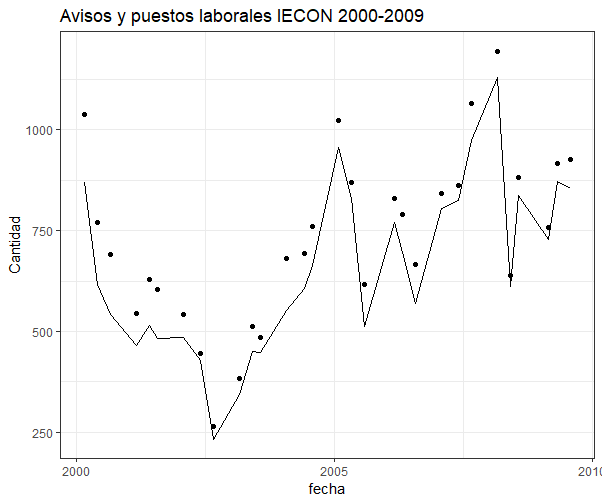
\includegraphics[width=\linewidth]{imagenes/chap4/iecon2000.png}
%		\caption{Avisos y Puestos IECON}
%	\end{subfigure}
%	\begin{subfigure}[b]{0.4\linewidth}
%		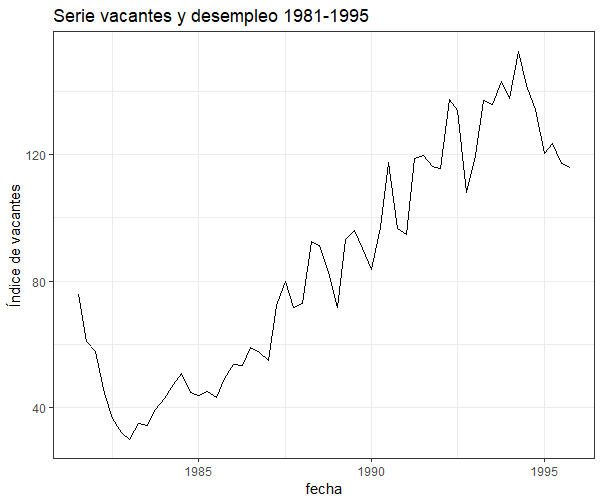
\includegraphics[width=\linewidth]{imagenes/chap4/VacantesUrrestarazu.png}
%		\caption{Vacantes Urrestarazu}
%	\end{subfigure}
%	\begin{subfigure}[b]{0.4\linewidth}
%		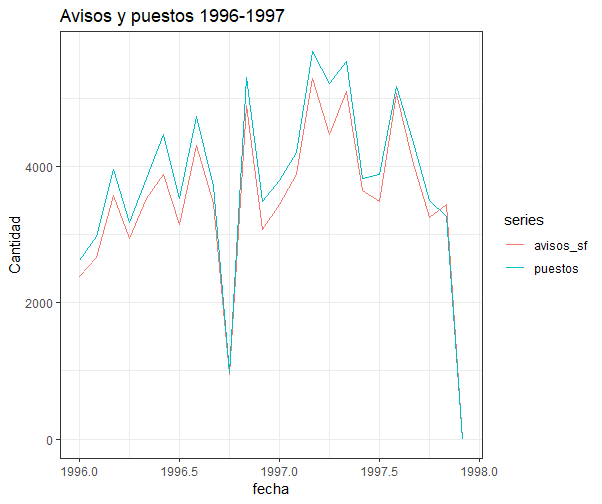
\includegraphics[width=\linewidth]{imagenes/chap4/MolinaAvisosyPuestos96.png}
%		\caption{Avisos recolectados 96-98}
%	\end{subfigure}
%	\begin{subfigure}[b]{0.4\linewidth}
%	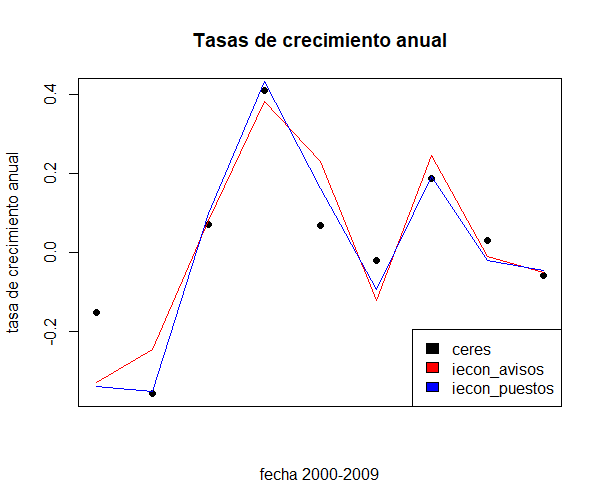
\includegraphics[width=\linewidth]{imagenes/chap4/CeresIECON2000.png}
%	\caption{Tasas crecimiento CERES-IECON}
%\end{subfigure}
%	\begin{subfigure}[b]{0.5\linewidth}
%		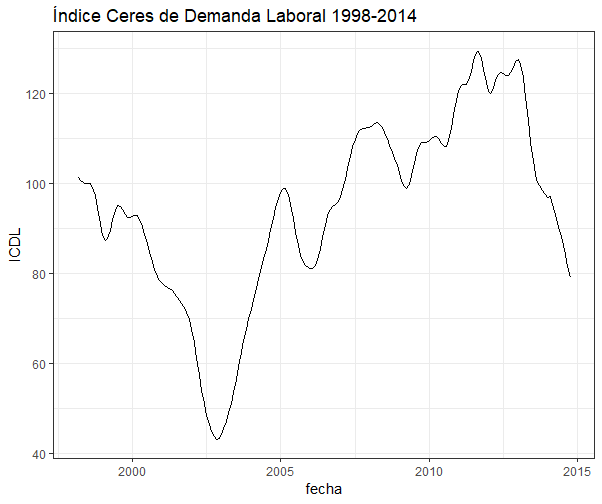
\includegraphics[width=\linewidth]{imagenes/chap4/ICDL98.png}
%		\caption{ICDL 1998-2014}
%	\end{subfigure}
%	\caption{Análisis de los datos obtenidos}
%	\label{fig:vacantes}
%\end{figure}

% PROBLEMÁTICAS

La serie de vacantes en proceso de construcción no esta exenta de críticas, las cuales vale destacar. La primera es que los datos solo permiten realizar un análisis para Montevideo, sin embargo, se encuentran sistemáticamente avisos laborales de otros departamentos del interior\footnote{Uruguay se compone de 19 grandes divisiones geográficas denominadas ``departamentos''. Por un lado esta Montevideo, y por el otro el resto de los 18 departamentos del país, lo que se denomina ``interior''.}, en especial de Maldonado y Canelones. Para el periodo recabado de 1995 a 1998 no se identifica cuantos avisos son y no son de Montevideo, sin embargo, si se logra obtener dicho número para el periodo de 2013-2018. En dicho caso los avisos publicados de otros departamentos oscilan en torno al 5\% del total publicaciones laborales. 

En segundo lugar, existe un claro sesgo hacia puestos laborales de baja calificación, lo cual se logra observar para el periodo 2013-2018 en base al análisis conjunto de la figura 2 y 3, donde se observa claramente que la mayor cantidad de avisos corresponden a puestos de auxiliar, técnico/especialista, ejecutivo comercial y peón. Esto va en linea con el resultado obtenido por \cite{Alma2011} para el periodo 2000-2010 utilizando la misma fuente de datos, quienes realizar un análisis pormenorizado de la información publicada en cada aviso laboral. Por lo cual, se supone que dicho sesgo también existe para el periodo 1980-1996.

%\begin{figure}[h]
%	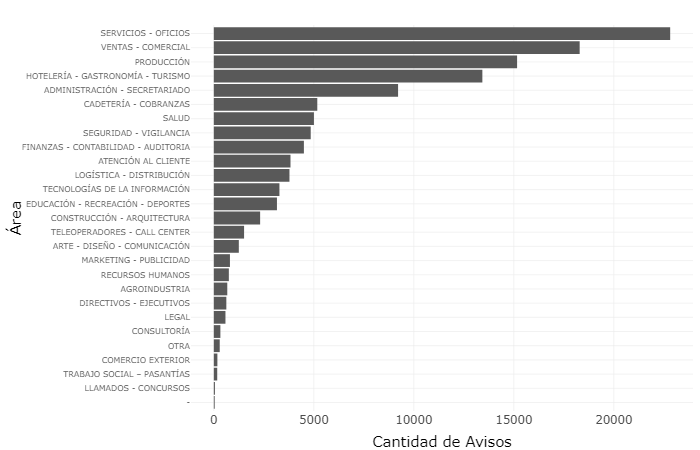
\includegraphics[width=\linewidth]{imagenes/chap4/newplot.png}
%	\caption{Cantidad de avisos laborales publicados en el diario El País, sección avisos laborales ``El Gallito'' entre 2013 y 2018. Los mismos son agrupados y ordenados de forma decreciente según el área en que se solicitan los avisos. El área, es una categoría propia del diario El País.}
%\end{figure}
%
%\begin{figure}[h]
%	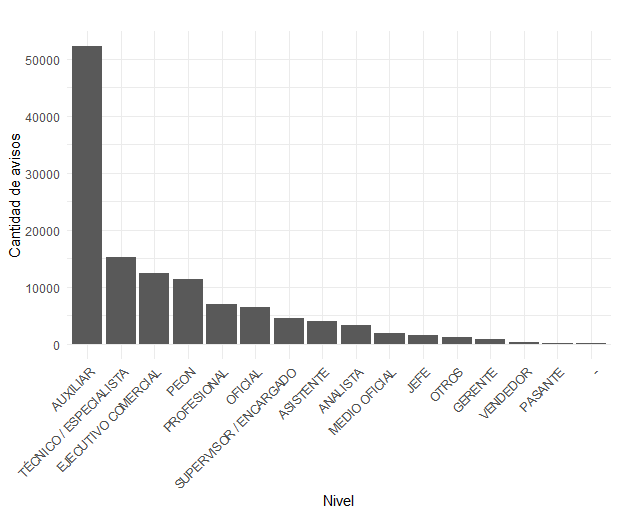
\includegraphics[width=\linewidth]{imagenes/chap4/gallito_nivel_2013_2018.png}
%	\caption{Cantidad de avisos laborales publicados en el diario El País, sección avisos laborales ``El Gallito'' entre 2013 y 2018. Los mismos son agrupados y ordenados de forma decreciente según el nivel jerárquico en que se solicitan los avisos. El nivel jerárquico, es una categoría propia del diario El País.}
%\end{figure}

En tercer lugar, la existencia de informalidad es una característica propia de los países subdesarrollados a la cual Uruguay y en específico Montevideo no escapa. Ello se agrava para los años entre 1980 y 2005, debido a las graves crisis económicas de 1982 y 2001-2002. Claramente las vacantes laborales publicadas en la prensa no captan los puestos generados en la informalidad.

Por último, ``El Gallito'' ha sido al menos hasta 2000-2010 el lugar predilecto por las empresas para publicar sus avisos laborales. Es un hecho incuestionable, por lo cual tomarlo como una muestra representativa de avisos laborales formales para el departamento de Montevideo es razonable. Sin embargo, con la penetración de Internet y la creación de portales de anuncios laborales como ``buscojobs'', ``computrabajo'', ``neuvo'' y ``linkedin'', entre otros, la competencia en el mercado de publicaciones ha aumentando considerablemente, no quedando claro en la actualidad cual es la página que reúne la mayor cantidad de avisos. Por esta razón, la representatividad del gallito ha disminuido y ello debe ser tenido en cuenta en el análisis, al menos desde 2009-2010 en adelante, dada la inserción de ``buscojobs'', ``computrabajo'' en torno a los años 2006-2007.

%\subsection{Estadísticas Descriptivas}

%[Presentar estadísticas descriptivas de los datos. Gráficos de las series, y al ser series temporales análisis estadísticas básicas de las series tales como test de R.U, de Raíz estacional, desestacionalización,]
 % Se carga el capítulo 04
  \chapter{Consideraciones finales}

En este capítulo se sintetizan las posturas expuestas en el capítulo anterior. Se retoma la pregunta de investigación y se expresa si los resultados apoyan o no la hipótesis planteada. 

Además, se pueden hacer contribuciones teóricas o metodológicas a la disciplina y recomendaciones para trabajos futuros o para profundizar en el campo, plantear nuevas interrogantes o proponer explicaciones \textit{post hoc}. En algunos trabajos este capítulo se subdivide en otras secciones que presentan algunos de los contenidos mencionados. 
En algunas tradiciones académicas este capítulo recibe distintas denominaciones: \textit{Conclusiones}, \textit{Conclusiones y trabajos a futuro}, \textit{Consideraciones finales y recomendaciones}. 

 % Se carga el capítulo 05
 % Seguir copiando la linea de arriba para agregar más capítulos.
  
  \backmatter % Comando que generalos apéndices, anexos y bibliografía. NO COMENTAR
  
  \bibliography{bibliografia/biblio_1,bibliografia/biblio_2,bibliografia/TesisBeveridgeCurve} % Agregar la cantidad de archivos .bib que se tengan para la bibliografía.
  \bibend % No comentar
  % 
  \glosario 		         % Glosario, NO comentar
  %
  \apenarabicnumbering
  \apenmatter				 % Apéndices, NO comentar
  \chapter{Datos procesados}


  \chapter{Imágenes remasterizadas}\label{Ape2}

  \chapter{Entrevistas desgrabadas}\label{Ape3}

  % Seguir copiando la linea de arriba para agregar más apéndices.
  %
  \anexarabicnumbering
  \anexmatter				 % Anexos, NO comentar
%  \chapter{Material legislativo}\label{Ane1}

XXXXX
  % Seguir copiando la linea de arriba para agregar más anexos.
  % 
\end{document}

% ===== FIN DEL DOCUMENTO =====
